\noindent\begin{minipage}{7cm}
\begin{description}
\item[Objectif :] comprendre la structure générale des tests (test simple, alternative simple, alternative multiple).
\item[Syntaxe \python :] \mbox{}
\begin{itemize}
\item \texttt{if condition : blocIf}
\item \texttt{if condition : blocIf}\\\texttt{else : blocElse}
\item \texttt{if condition : blocIf}\\\texttt{elif condition1 : blocElif1}\\\texttt{elif condition2 : blocElif2}\\\texttt{\ldots}\\\texttt{else : blocElse}
\end{itemize}
\end{description}
\end{minipage}
\mbox{}\hfill
\begin{tabular}{c}
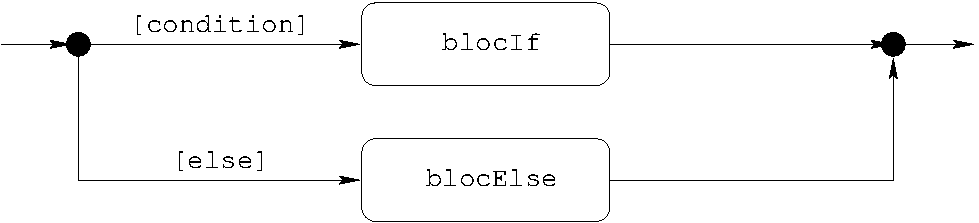
\includegraphics[width=6.5cm]{uml1.pdf}\\[3mm]
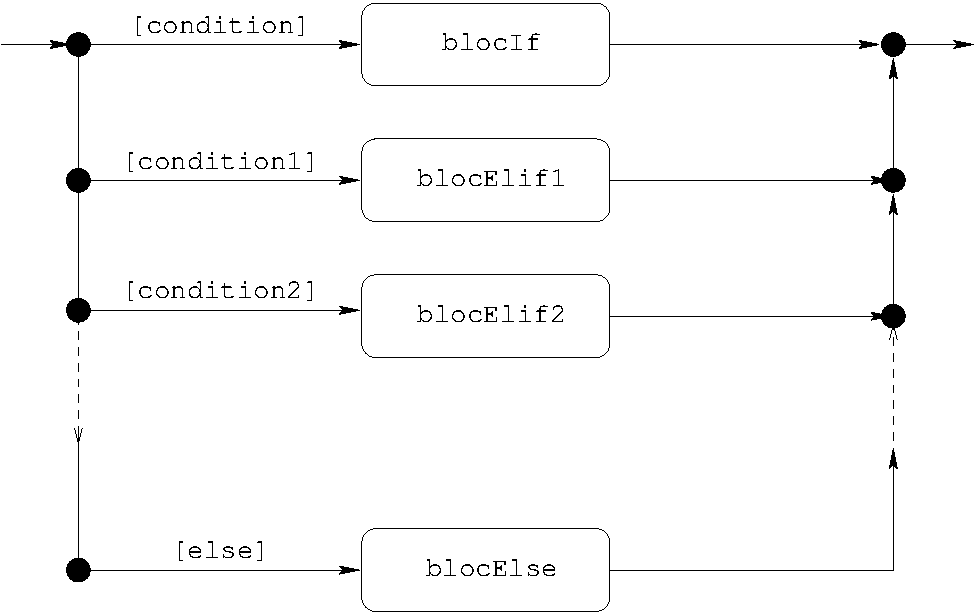
\includegraphics[width=6.5cm]{uml3.pdf}
\end{tabular}

%-------------------------------------------------------------------------
\subsection{Exemple}
%-------------------------------------------------------------------------

\paragraph{Enoncé :} on veut déterminer la mention au baccalauréat compte tenu
de la moyenne générale obtenue à l'examen.

\paragraph{Méthode :} on utilisera une alternative multiple.

\paragraph{Questions :} \mbox{}

\begin{question}[«~mentions au bac~» : graphe] Représenter par un graphe la relation 
$m = f(n)$
entre la mention $m$ ($m \in \{$insuffisant, passable, assez bien, bien, très bien$\}$) 
et la note $n$ obtenue ($n \in [0;20]$).
\end{question}

Le test simple est une instruction de contrôle du flux d'instructions 
qui permet d'exécuter une instruction sous condition préalable.
L'alternative simple est une instruction de contrôle du flux d'instructions 
qui permet de choisir entre deux instructions selon qu'une condition est vérifiée ou non.
L'alternative multiple est une instruction de contrôle du flux d'instructions 
qui permet de choisir entre plusieurs instructions en cascadant des alternatives simples.

\begin{question}[«~mentions au bac~» : alternative multiple] Ecrire une alternative multiple
qui calcule la mention en fonction de la note.
\end{question}


%-------------------------------------------------------------------------
\subsection{Généralisation}
%-------------------------------------------------------------------------
\begin{question}[alternatives : tests ou alternative ?]
Montrer à l'aide d'un contre-exemple que la séquence de tests simples (1)
n'est pas équivalente à l'alternative simple (2).

\noindent\begin{minipage}[t]{6cm}\footnotesize
\begin{enumerate}
\item \tt
\begin{Verbatim}
if condition : blocIf
if not condition : blocElse
\end{Verbatim}
\end{enumerate}
\end{minipage}
\hfill
\begin{minipage}[t]{6cm}\footnotesize
\begin{enumerate}\setcounter{enumi}{1}
\item \tt
\begin{Verbatim}
if condition : blocIf
else : blocElse
\end{Verbatim}
\end{enumerate}
\end{minipage}
\end{question}

\begin{question}[alternatives : multiples ou imbriquées ?]
Montrer à l'aide d'un contre-exemple que l'alternative multiple (1)
n'est pas équivalente à l'alternative multiple (2).
Donner leur équivalent à l'aide d'alternatives simples imbriquées.


\noindent\begin{minipage}[t]{6cm}\footnotesize
\begin{enumerate}
\item \tt
\begin{Verbatim}
if condition : blocIf
elif condition1 : blocElif1
elif condition2 : blocElif2
elif condition3 : blocElif3
else : blocElse
\end{Verbatim}
\end{enumerate}
\end{minipage}
\hfill
\begin{minipage}[t]{6cm}\footnotesize
\begin{enumerate}\setcounter{enumi}{1}
\item \tt
\begin{Verbatim}
if condition : blocIf
elif condition1 : blocElif1
elif condition3 : blocElif3
elif condition2 : blocElif2
else : blocElse
\end{Verbatim}
\end{enumerate}
\end{minipage}


\end{question}
%-------------------------------------------------------------------------
\subsection{Applications}
%-------------------------------------------------------------------------

\begin{question}[catégories sportives]
Ecrire un algorithme qui détermine la catégorie sportive d'un enfant selon
son âge : 
\begin{itemize}
\item Poussin de 6 à 7 ans,
\item Pupille de 8 à 9 ans,
\item Minime de 10 à 11 ans,
\item Cadet de 12 ans à 14 ans.
\end{itemize}
\end{question}


\begin{question}[prix d'une photocopie]
Ecrire un algorithme qui affiche le prix de $n$ photocopies sachant que
le reprographe facture 0,10 \euro{} les dix premières photocopies, 0,09 \euro{} 
	les vingt suivantes et 0,08 \euro{} au-delà.
\end{question}

\begin{question}[exécution d'une séquence de tests]\mbox{}

\noindent\begin{minipage}[t]{7cm}
\begin{enumerate}
\item Quelle est la valeur de la variable $ok$ après la suite
	d'instructions suivante ?

\footnotesize\tt\begin{Verbatim}
x = 2
y = 3
d = 5
h = 4
if x > 0 and x < d :
    if y > 0 and y < h : ok = 1
    else : ok = 0
else : ok = 0
\end{Verbatim}
\end{enumerate}
\end{minipage}
\begin{minipage}[t]{7cm}
\begin{enumerate}\setcounter{enumi}{1}
\item Quelle est la valeur de la variable $y$ après la suite
	d'instructions suivante ?

\footnotesize\tt\begin{Verbatim}
x = 3
y = -2
if x < y : y = y - x
elif x == y : y = 0
else : y = x - y
\end{Verbatim}
\end{enumerate}
\end{minipage}


\end{question}


%-------------------------------------------------------------------------
%\newpage
\subsection{Entraînement}
%-------------------------------------------------------------------------

%-------------------------------------------------------------------------
\subsubsection{Enoncé}
%-------------------------------------------------------------------------

\paragraph{Objectif :} calculer une fonction $y = f(x)$
définie par son graphe.

\paragraph{Méthode :} utiliser l'alternative multiple.

\paragraph{Vérification :} vérifier le bon fonctionnement sous \python{} en testant des points
caractéristiques de la fonction.

%-------------------------------------------------------------------------
\subsubsection{Exemple}
%-------------------------------------------------------------------------
On considère la fonction $y = f(x)$ 
définie sur $[-5;5]$  par le graphe ci-dessous et $\forall x < -5, f(x) = f(-5)$
et $\forall x > 5, f(x) = f(5)$. 

$$\begin{minipage}{6.75cm}
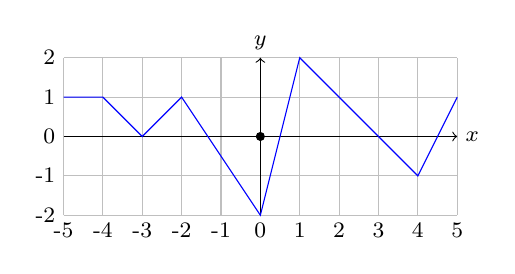
\begin{tikzpicture}[scale=0.5]\footnotesize
\draw[color=lightgray](-5,-2) grid[xstep=1,ystep=1] (5,2);
\foreach \x in {-5,-4,...,5} \draw(\x,-2) node[below]{\x};
\foreach \y in {-2,-1,...,2} \draw(-5,\y) node[left]{\y};
\filldraw(0,0) circle (0.1);
\draw[->] (-5,0) -- (5,0);
\draw (5,0) node[right]{$x$} ;
\draw[->] (0,-2) -- (0,2);
\draw (0,2) node[above]{$y$};
\draw[color=blue] (-5,1) -- (-4,1) -- (-3,0) -- (-2,1) -- (0,-2) -- (1,2) -- (4,-1) -- (5,1);
%\draw (-4.5,1) node[above]{\Pisymbol{pzd}{172}};
%\draw (-3.5,0.5) node[above]{\Pisymbol{pzd}{173}};
%\draw (-2.5,0.5) node[below]{\Pisymbol{pzd}{174}};
%\draw (-1,-0.5) node[below]{\Pisymbol{pzd}{175}};
%\draw (0.5,0) node[right]{\Pisymbol{pzd}{176}};
%\draw (2.5,0.5) node[right]{\Pisymbol{pzd}{177}};
%\draw (4.5,0) node[above]{\Pisymbol{pzd}{178}};
\end{tikzpicture}
\end{minipage}
$$

\paragraph{Méthode :} 
Lorsqu'on connaît 2 points $M(x_M,y_M)$ et $N(x_N,y_N)$ 
d'une droite d'équation $y = ax + b$, les coefficients $a$ (pente de la droite) 
et $b$ (ordonnée à l'origine) de la droite sont obtenus
par résolution du système de 2 équations : $y_M =ax_M + b$ et $y_N = ax_N + b$. 
On obtient alors $a$ et $b$ :

$$\begin{minipage}{6.75cm}
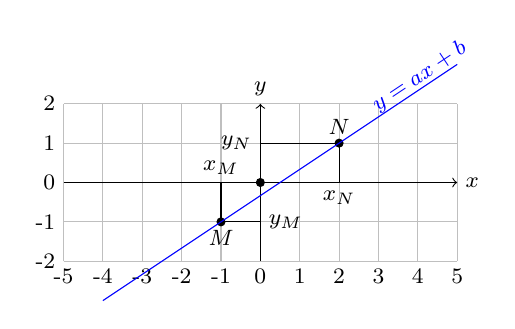
\begin{tikzpicture}[scale=0.5]\footnotesize
\draw[color=lightgray](-5,-2) grid[xstep=1,ystep=1] (5,2);
\foreach \x in {-5,-4,...,5} \draw(\x,-2) node[below]{\x};
\foreach \y in {-2,-1,...,2} \draw(-5,\y) node[left]{\y};
\filldraw(0,0) circle (0.1);
\filldraw(-1,-1) circle (0.1);
\draw (-1,-1) node[below]{$M$};
\draw(-1,0) node[above]{$x_M$};
\draw(0,-1) node[right]{$y_M$};
\draw (-1,-1) -- (-1,0);
\draw (-1,-1) -- (0,-1);
\filldraw(2,1) circle (0.1);
\draw (2,1) node[above]{$N$};
\draw(2,0) node[below]{$x_N$};
\draw(0,1) node[left]{$y_N$};
\draw (2,1) -- (2,0);
\draw (2,1) -- (0,1);
\draw[->] (-5,0) -- (5,0);
\draw (5,0) node[right]{$x$} ;
\draw[->] (0,-2) -- (0,2);
\draw (0,2) node[above]{$y$};
\draw[color=blue] (-4,-3) -- (5,3);
\draw[color=blue](4.3,2.3) node[above,rotate=33.69]{$y = ax + b$};
\end{tikzpicture}
\end{minipage}
\hfill
\begin{minipage}{8.75cm}
$$\displaystyle a = \frac{y_N - y_M}{x_N - x_M} \mbox{ et } \displaystyle b = \frac{y_Mx_N - y_Nx_M}{x_N - x_M}$$
Pour la droite ci-contre :
$$\displaystyle 
a = \frac{1 - (-1)}{2 - (-1)} = \frac{2}{3} \mbox{ et } \displaystyle 
b = \frac{(-1)\cdot 2 - 1\cdot(-1)}{2 - (-1)} = -\frac{1}{3}
$$
On vérifie graphiquement ces résultats : pour passer de $M$ à $N$, on
se déplace de 3 horizontalement puis de 2 verticalement (d'où la pente $a = 2/3$),
et la droite coupe bien l'axe des ordonnées en $y = -1/3$.
\end{minipage}$$

Il faut donc déterminer les équations de droite 
correspondant aux différents segments du graphe de la fonction, à savoir :
$$\begin{minipage}{9cm}
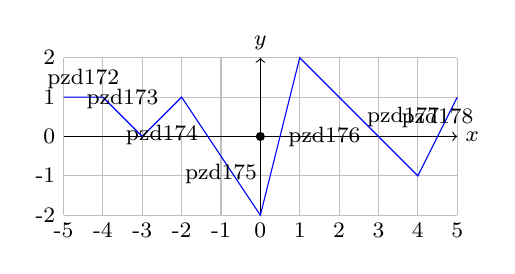
\begin{tikzpicture}[scale=0.5]\footnotesize
\draw[color=lightgray](-5,-2) grid[xstep=1,ystep=1] (5,2);
\foreach \x in {-5,-4,...,5} \draw(\x,-2) node[below]{\x};
\foreach \y in {-2,-1,...,2} \draw(-5,\y) node[left]{\y};
\filldraw(0,0) circle (0.1);
\draw[->] (-5,0) -- (5,0);
\draw (5,0) node[right]{$x$} ;
\draw[->] (0,-2) -- (0,2);
\draw (0,2) node[above]{$y$};
\draw[color=blue] (-5,1) -- (-4,1) -- (-3,0) -- (-2,1) -- (0,-2) -- (1,2) -- (4,-1) -- (5,1);
\draw (-4.5,1) node[above]{\Pisymbol{pzd}{172}};
\draw (-3.5,0.5) node[above]{\Pisymbol{pzd}{173}};
\draw (-2.5,0.5) node[below]{\Pisymbol{pzd}{174}};
\draw (-1,-0.5) node[below]{\Pisymbol{pzd}{175}};
\draw (0.5,0) node[right]{\Pisymbol{pzd}{176}};
\draw (2.5,0.5) node[right]{\Pisymbol{pzd}{177}};
\draw (4.5,0) node[above]{\Pisymbol{pzd}{178}};
\end{tikzpicture}
\end{minipage}
\hfill
\begin{minipage}{3cm}
\begin{itemize}
\item[\Pisymbol{pzd}{172}] $y = 1$
\item[\Pisymbol{pzd}{173}] $y = -x -3$
\item[\Pisymbol{pzd}{174}] $y = x + 3$
\item[\Pisymbol{pzd}{175}] $y = -3x/2 - 2$
\item[\Pisymbol{pzd}{176}] $y = 4x - 2$
\item[\Pisymbol{pzd}{177}] $y = -x + 3$
\item[\Pisymbol{pzd}{178}] $y = 2x - 9$
\end{itemize}
\end{minipage}$$
\vspace*{2mm}

\noindent
\begin{minipage}[t]{7cm}
\paragraph{Résultat :} Compte-tenu de ces équations, le code ci-contre
permet de calculer $y = f(x)$, y compris pour $x < -5$ et $x > 5$.
Pour le tester, on comparera les valeurs obtenues par le calcul avec celles lues
directement sur le graphe pour quelques points caractéristiques.
\end{minipage}
\hfill
\begin{minipage}[t]{8cm}
\begin{lstlisting}
if   x < -4 : y = 1
elif x < -3 : y = -x - 3
elif x < -2 : y = x + 3
elif x <  0 : y = -3*x/2 - 2
elif x <  1 : y = 4*x - 2
elif x <  4 : y = -x + 3
elif x <  5 : y = 2*x - 9
else        : y = 1
\end{lstlisting}
\end{minipage}

\newpage
\paragraph{Vérifications :} 
On peut vérifier par exemple pour $x = -1$ 
($\rightarrow y = -0.5$) et $x = 3$ ($\rightarrow y = 0$).

$$\begin{minipage}{6.5cm}\footnotesize
\begin{Verbatim}
>>> x = -1
>>> if   x < -4 : y = 1
elif x < -3 : y = -x - 3
elif x < -2 : y = x + 3
elif x <  0 : y = -3*x/2 - 2
elif x <  1 : y = 4*x - 2
elif x <  4 : y = -x + 3
elif x <  5 : y = 2*x - 9
else        : y = 1

>>> y
-0.5
\end{Verbatim}
\end{minipage}
\hfill
\begin{minipage}{6.5cm}\footnotesize
\begin{Verbatim}
>>> x = 3
>>> if   x < -4 : y = 1
elif x < -3 : y = -x - 3
elif x < -2 : y = x + 3
elif x <  0 : y = -3*x/2 - 2
elif x <  1 : y = 4*x - 2
elif x <  4 : y = -x + 3
elif x <  5 : y = 2*x - 9
else        : y = 1

>>> y
0
\end{Verbatim}
\end{minipage}$$

%-------------------------------------------------------------------------
\subsubsection{Questions}
%-------------------------------------------------------------------------
Ecrire une alternative multiple qui permette
de déterminer $y = f(x)$ pour une fonction $f$ définie par son graphe
sur $[-5;5]$ et $\forall x < -5, f(x) = f(-5)$
et $\forall x > 5, f(x) = f(5)$.

\noindent\begin{minipage}{7.75cm}
\begin{enumerate}
\item \begin{minipage}{6.75cm}
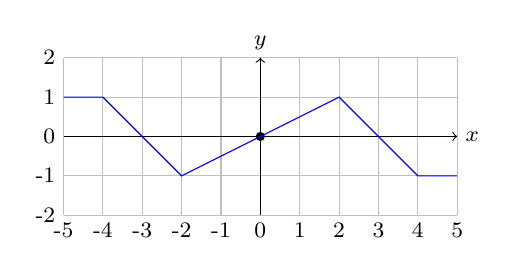
\begin{tikzpicture}[scale=0.5]\footnotesize
\draw[color=lightgray](-5,-2) grid[xstep=1,ystep=1] (5,2);
\foreach \x in {-5,-4,...,5} \draw(\x,-2) node[below]{\x};
\foreach \y in {-2,-1,...,2} \draw(-5,\y) node[left]{\y};
\filldraw(0,0) circle (0.1);
\draw[->] (-5,0) -- (5,0);
\draw (5,0) node[right]{$x$} ;
\draw[->] (0,-2) -- (0,2);
\draw (0,2) node[above]{$y$};
\draw[color=blue] (-5,1) -- (-4,1) -- (-2,-1) -- (2,1) -- (4,-1) -- (5,-1);
\end{tikzpicture}
\end{minipage}

\item \begin{minipage}{6.75cm}
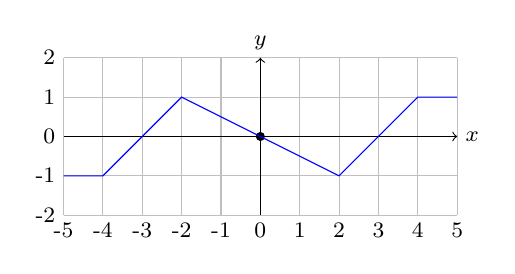
\begin{tikzpicture}[scale=0.5]\footnotesize
\draw[color=lightgray](-5,-2) grid[xstep=1,ystep=1] (5,2);
\foreach \x in {-5,-4,...,5} \draw(\x,-2) node[below]{\x};
\foreach \y in {-2,-1,...,2} \draw(-5,\y) node[left]{\y};
\filldraw(0,0) circle (0.1);
\draw[->] (-5,0) -- (5,0); 
\draw (5,0) node[right]{$x$} ;
\draw[->] (0,-2) -- (0,2);
\draw (0,2) node[above]{$y$};
\draw[color=blue] (-5,-1) -- (-4,-1) -- (-2,1) -- (2,-1) -- (4,1) -- (5,1);
\end{tikzpicture}
\end{minipage}

\item \begin{minipage}{6.75cm}
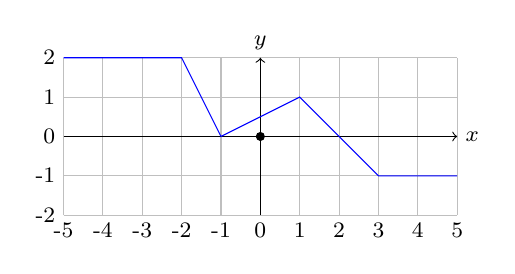
\begin{tikzpicture}[scale=0.5]\footnotesize
\draw[color=lightgray](-5,-2) grid[xstep=1,ystep=1] (5,2);
\foreach \x in {-5,-4,...,5} \draw(\x,-2) node[below]{\x};
\foreach \y in {-2,-1,...,2} \draw(-5,\y) node[left]{\y};
\filldraw(0,0) circle (0.1);
\draw[->] (-5,0) -- (5,0);
\draw (5,0) node[right]{$x$} ;
\draw[->] (0,-2) -- (0,2);
\draw (0,2) node[above]{$y$};
\draw[color=blue] (-5,2) -- (-2,2) -- (-1,0) -- (1,1) -- (3,-1) -- (5,-1);
\end{tikzpicture}
\end{minipage}

\item \begin{minipage}{6.75cm}
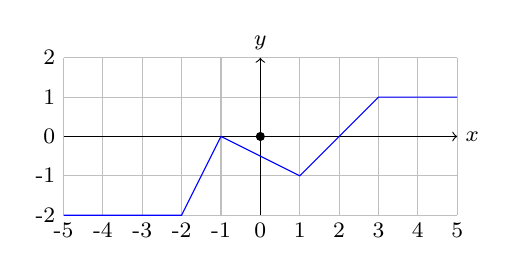
\begin{tikzpicture}[scale=0.5]\footnotesize
\draw[color=lightgray](-5,-2) grid[xstep=1,ystep=1] (5,2);
\foreach \x in {-5,-4,...,5} \draw(\x,-2) node[below]{\x};
\foreach \y in {-2,-1,...,2} \draw(-5,\y) node[left]{\y};
\filldraw(0,0) circle (0.1);
\draw[->] (-5,0) -- (5,0); 
\draw (5,0) node[right]{$x$} ;
\draw[->] (0,-2) -- (0,2);
\draw (0,2) node[above]{$y$};
\draw[color=blue] (-5,-2) -- (-2,-2) -- (-1,0) -- (1,-1) -- (3,1) -- (5,1);
\end{tikzpicture}
\end{minipage}

\item \begin{minipage}{6.75cm}
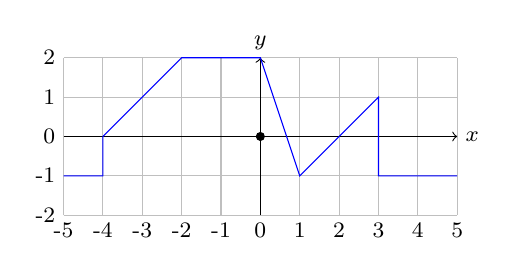
\begin{tikzpicture}[scale=0.5]\footnotesize
\draw[color=lightgray](-5,-2) grid[xstep=1,ystep=1] (5,2);
\foreach \x in {-5,-4,...,5} \draw(\x,-2) node[below]{\x};
\foreach \y in {-2,-1,...,2} \draw(-5,\y) node[left]{\y};
\filldraw(0,0) circle (0.1);
\draw[->] (-5,0) -- (5,0);
\draw (5,0) node[right]{$x$} ;
\draw[->] (0,-2) -- (0,2);
\draw (0,2) node[above]{$y$};
\draw[color=blue] (-5,-1) -- (-4,-1) -- (-4,0) -- (-2,2) -- (0,2) -- (1,-1) -- (1,-1) -- (3,1) -- (3,-1) -- (5,-1);
\end{tikzpicture}
\end{minipage}

\end{enumerate}
\end{minipage}
\hfill
\begin{minipage}{7.75cm}
\begin{enumerate}\setcounter{enumi}{5}

\item \begin{minipage}{6.75cm}
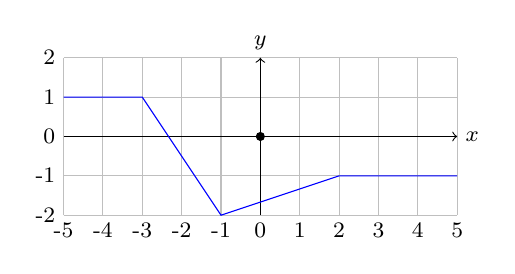
\begin{tikzpicture}[scale=0.5]\footnotesize
\draw[color=lightgray](-5,-2) grid[xstep=1,ystep=1] (5,2);
\foreach \x in {-5,-4,...,5} \draw(\x,-2) node[below]{\x};
\foreach \y in {-2,-1,...,2} \draw(-5,\y) node[left]{\y};
\filldraw(0,0) circle (0.1);
\draw[->] (-5,0) -- (5,0); 
\draw (5,0) node[right]{$x$} ;
\draw[->] (0,-2) -- (0,2);
\draw (0,2) node[above]{$y$};
\draw[color=blue] (-5,1) -- (-3,1) -- (-1,-2) -- (2,-1) -- (4,-1) -- (5,-1);
\end{tikzpicture}
\end{minipage}

\item \begin{minipage}{6.75cm}
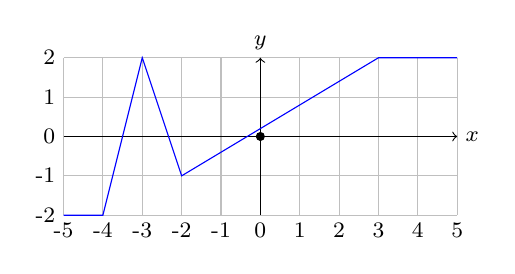
\begin{tikzpicture}[scale=0.5]\footnotesize
\draw[color=lightgray](-5,-2) grid[xstep=1,ystep=1] (5,2);
\foreach \x in {-5,-4,...,5} \draw(\x,-2) node[below]{\x};
\foreach \y in {-2,-1,...,2} \draw(-5,\y) node[left]{\y};
\filldraw(0,0) circle (0.1);
\draw[->] (-5,0) -- (5,0);
\draw (5,0) node[right]{$x$} ;
\draw[->] (0,-2) -- (0,2);
\draw (0,2) node[above]{$y$};
\draw[color=blue] (-5,-2) -- (-4,-2) -- (-3,2) -- (-2,-1) -- (3,2) -- (5,2);
\end{tikzpicture}
\end{minipage}

\item \begin{minipage}{6.75cm}
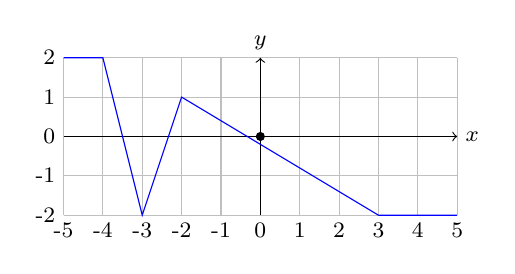
\begin{tikzpicture}[scale=0.5]\footnotesize
\draw[color=lightgray](-5,-2) grid[xstep=1,ystep=1] (5,2);
\foreach \x in {-5,-4,...,5} \draw(\x,-2) node[below]{\x};
\foreach \y in {-2,-1,...,2} \draw(-5,\y) node[left]{\y};
\filldraw(0,0) circle (0.1);
\draw[->] (-5,0) -- (5,0); 
\draw (5,0) node[right]{$x$} ;
\draw[->] (0,-2) -- (0,2);
\draw (0,2) node[above]{$y$};
\draw[color=blue] (-5,2) -- (-4,2) -- (-3,-2) -- (-2,1) -- (3,-2) -- (5,-2);
\end{tikzpicture}
\end{minipage}

\item \begin{minipage}{6.75cm}
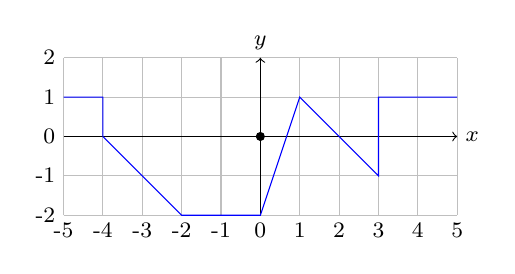
\begin{tikzpicture}[scale=0.5]\footnotesize
\draw[color=lightgray](-5,-2) grid[xstep=1,ystep=1] (5,2);
\foreach \x in {-5,-4,...,5} \draw(\x,-2) node[below]{\x};
\foreach \y in {-2,-1,...,2} \draw(-5,\y) node[left]{\y};
\filldraw(0,0) circle (0.1);
\draw[->] (-5,0) -- (5,0); 
\draw (5,0) node[right]{$x$} ;
\draw[->] (0,-2) -- (0,2);
\draw (0,2) node[above]{$y$};
\draw[color=blue] (-5,1) -- (-4,1) -- (-4,0) -- (-2,-2) -- (0,-2) -- (1,1) -- (1,1) -- (3,-1) -- (3,1) -- (5,1);
\end{tikzpicture}
\end{minipage}

\item \begin{minipage}{6.75cm}
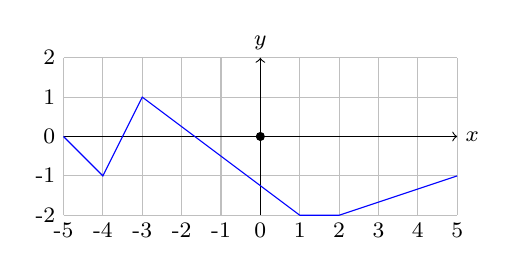
\begin{tikzpicture}[scale=0.5]\footnotesize
\draw[color=lightgray](-5,-2) grid[xstep=1,ystep=1] (5,2);
\foreach \x in {-5,-4,...,5} \draw(\x,-2) node[below]{\x};
\foreach \y in {-2,-1,...,2} \draw(-5,\y) node[left]{\y};
\filldraw(0,0) circle (0.1);
\draw[->] (-5,0) -- (5,0); 
\draw (5,0) node[right]{$x$} ;
\draw[->] (0,-2) -- (0,2);
\draw (0,2) node[above]{$y$};
\draw[color=blue] (-5,0) -- (-4,-1) -- (-3,1) -- (1,-2) -- (2,-2) -- (5,-1);
\end{tikzpicture}
\end{minipage}

\end{enumerate}
\end{minipage}

\noindent\begin{minipage}[t]{7.75cm}
\begin{enumerate}\setcounter{enumi}{10}

\item \begin{minipage}{6.75cm}
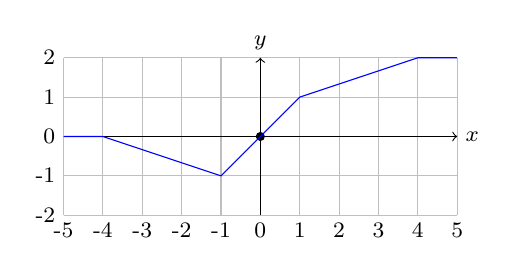
\begin{tikzpicture}[scale=0.5]\footnotesize
\draw[color=lightgray](-5,-2) grid[xstep=1,ystep=1] (5,2);
\foreach \x in {-5,-4,...,5} \draw(\x,-2) node[below]{\x};
\foreach \y in {-2,-1,...,2} \draw(-5,\y) node[left]{\y};
\filldraw(0,0) circle (0.1);
\draw[->] (-5,0) -- (5,0);
\draw (5,0) node[right]{$x$} ;
\draw[->] (0,-2) -- (0,2);
\draw (0,2) node[above]{$y$};
\draw[color=blue] (-5,0) -- (-4,0) -- (-1,-1) -- (1,1) -- (4,2) -- (5,2);
\end{tikzpicture}
\end{minipage}

\item \begin{minipage}{6.75cm}
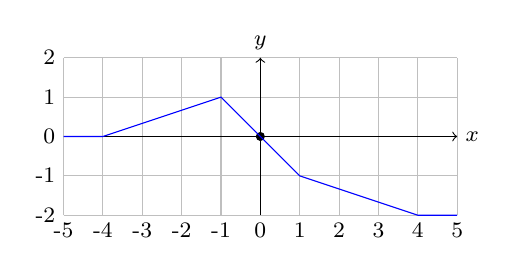
\begin{tikzpicture}[scale=0.5]\footnotesize
\draw[color=lightgray](-5,-2) grid[xstep=1,ystep=1] (5,2);
\foreach \x in {-5,-4,...,5} \draw(\x,-2) node[below]{\x};
\foreach \y in {-2,-1,...,2} \draw(-5,\y) node[left]{\y};
\filldraw(0,0) circle (0.1);
\draw[->] (-5,0) -- (5,0); 
\draw (5,0) node[right]{$x$} ;
\draw[->] (0,-2) -- (0,2);
\draw (0,2) node[above]{$y$};
\draw[color=blue] (-5,0) -- (-4,0) -- (-1,1) -- (1,-1) -- (4,-2) -- (5,-2);
\end{tikzpicture}
\end{minipage}

\item \begin{minipage}{6.75cm}
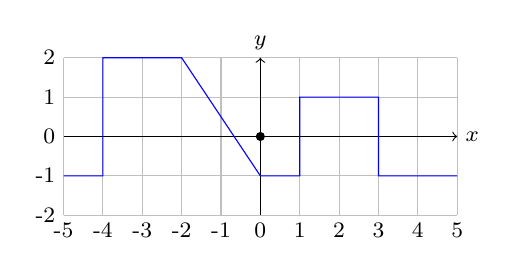
\begin{tikzpicture}[scale=0.5]\footnotesize
\draw[color=lightgray](-5,-2) grid[xstep=1,ystep=1] (5,2);
\foreach \x in {-5,-4,...,5} \draw(\x,-2) node[below]{\x};
\foreach \y in {-2,-1,...,2} \draw(-5,\y) node[left]{\y};
\filldraw(0,0) circle (0.1);
\draw[->] (-5,0) -- (5,0);
\draw (5,0) node[right]{$x$} ;
\draw[->] (0,-2) -- (0,2);
\draw (0,2) node[above]{$y$};
\draw[color=blue] (-5,-1) -- (-4,-1) -- (-4,2) -- (-2,2) -- (0,-1) -- (1,-1) -- (1,1) -- (3,1) -- (3,-1) -- (5,-1);
\end{tikzpicture}
\end{minipage}

\item \begin{minipage}{6.75cm}
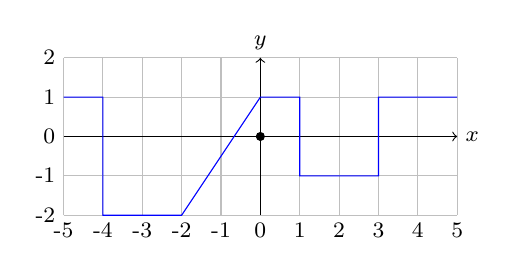
\begin{tikzpicture}[scale=0.5]\footnotesize
\draw[color=lightgray](-5,-2) grid[xstep=1,ystep=1] (5,2);
\foreach \x in {-5,-4,...,5} \draw(\x,-2) node[below]{\x};
\foreach \y in {-2,-1,...,2} \draw(-5,\y) node[left]{\y};
\filldraw(0,0) circle (0.1);
\draw[->] (-5,0) -- (5,0); 
\draw (5,0) node[right]{$x$} ;
\draw[->] (0,-2) -- (0,2);
\draw (0,2) node[above]{$y$};
\draw[color=blue] (-5,1) -- (-4,1) -- (-4,-2) -- (-2,-2) -- (0,1) -- (1,1) -- (1,-1) -- (3,-1) -- (3,1) -- (5,1);
\end{tikzpicture}
\end{minipage}

\item \begin{minipage}{6.75cm}
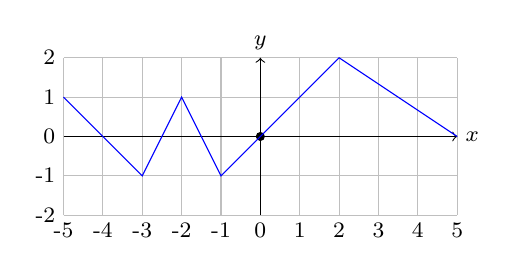
\begin{tikzpicture}[scale=0.5]\footnotesize
\draw[color=lightgray](-5,-2) grid[xstep=1,ystep=1] (5,2);
\foreach \x in {-5,-4,...,5} \draw(\x,-2) node[below]{\x};
\foreach \y in {-2,-1,...,2} \draw(-5,\y) node[left]{\y};
\filldraw(0,0) circle (0.1);
\draw[->] (-5,0) -- (5,0);
\draw (5,0) node[right]{$x$} ;
\draw[->] (0,-2) -- (0,2);
\draw (0,2) node[above]{$y$};
\draw[color=blue] (-5,1) -- (-3,-1) -- (-2,1) -- (-1,-1) -- (2,2) -- (5,0);
\end{tikzpicture}
\end{minipage}

\item \begin{minipage}{6.75cm}
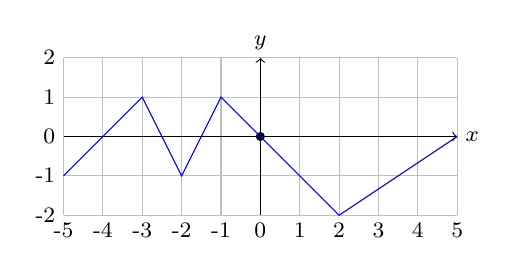
\begin{tikzpicture}[scale=0.5]\footnotesize
\draw[color=lightgray](-5,-2) grid[xstep=1,ystep=1] (5,2);
\foreach \x in {-5,-4,...,5} \draw(\x,-2) node[below]{\x};
\foreach \y in {-2,-1,...,2} \draw(-5,\y) node[left]{\y};
\filldraw(0,0) circle (0.1);
\draw[->] (-5,0) -- (5,0); 
\draw (5,0) node[right]{$x$} ;
\draw[->] (0,-2) -- (0,2);
\draw (0,2) node[above]{$y$};
\draw[color=blue] (-5,-1) -- (-3,1) -- (-2,-1) -- (-1,1) -- (2,-2) -- (5,0);
\end{tikzpicture}
\end{minipage}

\item \begin{minipage}{6.75cm}
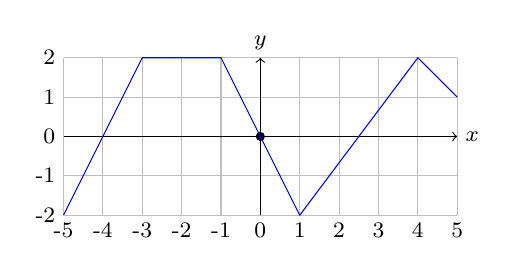
\begin{tikzpicture}[scale=0.5]\footnotesize
\draw[color=lightgray](-5,-2) grid[xstep=1,ystep=1] (5,2);
\foreach \x in {-5,-4,...,5} \draw(\x,-2) node[below]{\x};
\foreach \y in {-2,-1,...,2} \draw(-5,\y) node[left]{\y};
\filldraw(0,0) circle (0.1);
\draw[->] (-5,0) -- (5,0);
\draw (5,0) node[right]{$x$} ;
\draw[->] (0,-2) -- (0,2);
\draw (0,2) node[above]{$y$};
\draw[color=blue] (-5,-2) -- (-3,2) -- (-1,2) -- (1,-2) -- (4,2) -- (5,1);
\end{tikzpicture}
\end{minipage}

\end{enumerate}
\end{minipage}
\hfill
\begin{minipage}[t]{7.75cm}
\begin{enumerate}\setcounter{enumi}{17}

\item \begin{minipage}{6.75cm}
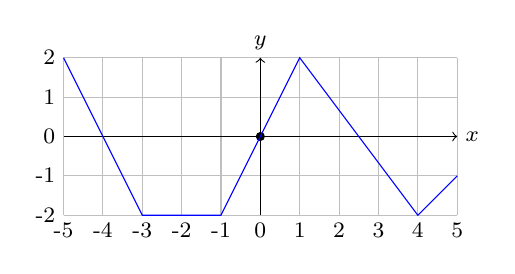
\begin{tikzpicture}[scale=0.5]\footnotesize
\draw[color=lightgray](-5,-2) grid[xstep=1,ystep=1] (5,2);
\foreach \x in {-5,-4,...,5} \draw(\x,-2) node[below]{\x};
\foreach \y in {-2,-1,...,2} \draw(-5,\y) node[left]{\y};
\filldraw(0,0) circle (0.1);
\draw[->] (-5,0) -- (5,0); 
\draw (5,0) node[right]{$x$} ;
\draw[->] (0,-2) -- (0,2);
\draw (0,2) node[above]{$y$};
\draw[color=blue] (-5,2) -- (-3,-2) -- (-1,-2) -- (1,2) -- (4,-2) -- (5,-1);
\end{tikzpicture}
\end{minipage}

\item \begin{minipage}{6.75cm}
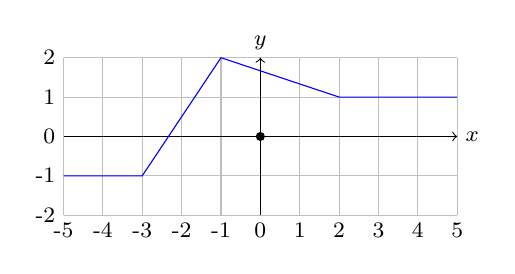
\begin{tikzpicture}[scale=0.5]\footnotesize
\draw[color=lightgray](-5,-2) grid[xstep=1,ystep=1] (5,2);
\foreach \x in {-5,-4,...,5} \draw(\x,-2) node[below]{\x};
\foreach \y in {-2,-1,...,2} \draw(-5,\y) node[left]{\y};
\filldraw(0,0) circle (0.1);
\draw[->] (-5,0) -- (5,0);
\draw (5,0) node[right]{$x$} ;
\draw[->] (0,-2) -- (0,2);
\draw (0,2) node[above]{$y$};
\draw[color=blue] (-5,-1) -- (-3,-1) -- (-1,2) -- (2,1) -- (4,1) -- (5,1);
\end{tikzpicture}
\end{minipage}

\item \begin{minipage}{6.75cm}
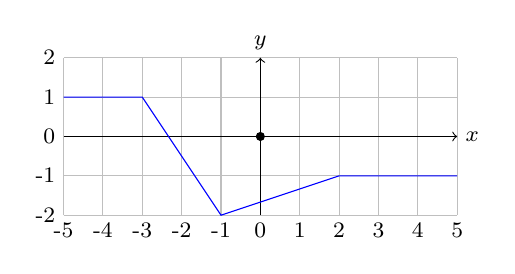
\begin{tikzpicture}[scale=0.5]\footnotesize
\draw[color=lightgray](-5,-2) grid[xstep=1,ystep=1] (5,2);
\foreach \x in {-5,-4,...,5} \draw(\x,-2) node[below]{\x};
\foreach \y in {-2,-1,...,2} \draw(-5,\y) node[left]{\y};
\filldraw(0,0) circle (0.1);
\draw[->] (-5,0) -- (5,0); 
\draw (5,0) node[right]{$x$} ;
\draw[->] (0,-2) -- (0,2);
\draw (0,2) node[above]{$y$};
\draw[color=blue] (-5,1) -- (-3,1) -- (-1,-2) -- (2,-1) -- (4,-1) -- (5,-1);
\end{tikzpicture}
\end{minipage}

\item \begin{minipage}{6.75cm}
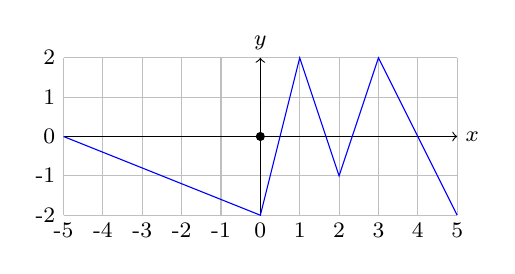
\begin{tikzpicture}[scale=0.5]\footnotesize
\draw[color=lightgray](-5,-2) grid[xstep=1,ystep=1] (5,2);
\foreach \x in {-5,-4,...,5} \draw(\x,-2) node[below]{\x};
\foreach \y in {-2,-1,...,2} \draw(-5,\y) node[left]{\y};
\filldraw(0,0) circle (0.1);
\draw[->] (-5,0) -- (5,0);
\draw (5,0) node[right]{$x$} ;
\draw[->] (0,-2) -- (0,2);
\draw (0,2) node[above]{$y$};
\draw[color=blue] (-5,0) -- (0,-2) -- (1,2) -- (2,-1) -- (3,2) -- (5,-2);
\end{tikzpicture}
\end{minipage}

\item \begin{minipage}{6.75cm}
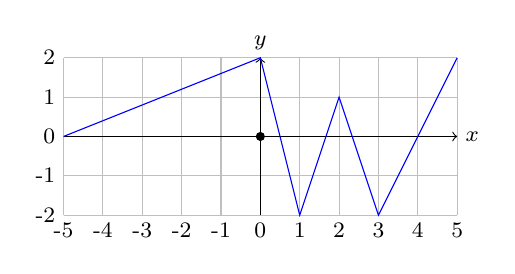
\begin{tikzpicture}[scale=0.5]\footnotesize
\draw[color=lightgray](-5,-2) grid[xstep=1,ystep=1] (5,2);
\foreach \x in {-5,-4,...,5} \draw(\x,-2) node[below]{\x};
\foreach \y in {-2,-1,...,2} \draw(-5,\y) node[left]{\y};
\filldraw(0,0) circle (0.1);
\draw[->] (-5,0) -- (5,0); 
\draw (5,0) node[right]{$x$} ;
\draw[->] (0,-2) -- (0,2);
\draw (0,2) node[above]{$y$};
\draw[color=blue] (-5,0) -- (0,2) -- (1,-2) -- (2,1) -- (3,-2) -- (5,2);
\end{tikzpicture}
\end{minipage}

\item \begin{minipage}{6.75cm}
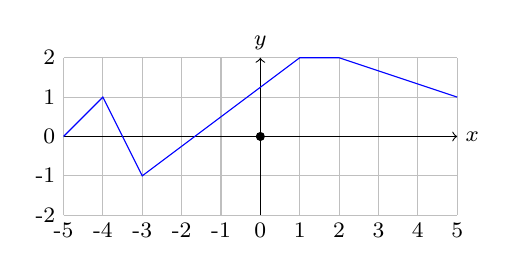
\begin{tikzpicture}[scale=0.5]\footnotesize
\draw[color=lightgray](-5,-2) grid[xstep=1,ystep=1] (5,2);
\foreach \x in {-5,-4,...,5} \draw(\x,-2) node[below]{\x};
\foreach \y in {-2,-1,...,2} \draw(-5,\y) node[left]{\y};
\filldraw(0,0) circle (0.1);
\draw[->] (-5,0) -- (5,0);
\draw (5,0) node[right]{$x$} ;
\draw[->] (0,-2) -- (0,2);
\draw (0,2) node[above]{$y$};
\draw[color=blue] (-5,0) -- (-4,1) -- (-3,-1) -- (1,2) -- (2,2) -- (5,1);
\end{tikzpicture}
\end{minipage}

\item \begin{minipage}{6.75cm}
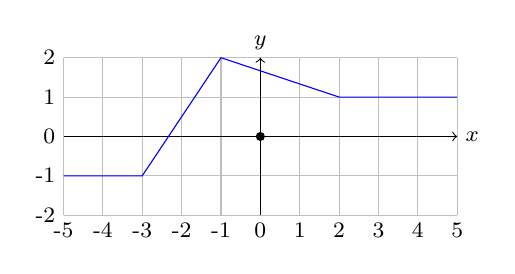
\begin{tikzpicture}[scale=0.5]\footnotesize
\draw[color=lightgray](-5,-2) grid[xstep=1,ystep=1] (5,2);
\foreach \x in {-5,-4,...,5} \draw(\x,-2) node[below]{\x};
\foreach \y in {-2,-1,...,2} \draw(-5,\y) node[left]{\y};
\filldraw(0,0) circle (0.1);
\draw[->] (-5,0) -- (5,0);
\draw (5,0) node[right]{$x$} ;
\draw[->] (0,-2) -- (0,2);
\draw (0,2) node[above]{$y$};
\draw[color=blue] (-5,-1) -- (-3,-1) -- (-1,2) -- (2,1) -- (4,1) -- (5,1);
\end{tikzpicture}
\end{minipage}

\end{enumerate}
\end{minipage}


%-------------------------------------------------------------------------
\subsection{Révisions}
%-------------------------------------------------------------------------

$$\begin{tabular}{|ll@{ : }l|}
\hline
\textbf{Cours} & \cite{cours} & chapitre 2, section 2.3 \\
\textbf{TD}    & \cite{td}    & exercices 2.8 à 2.11, 2.30 à 2.32 \\
\hline
\end{tabular}$$
